\documentclass[10pt,a4paper]{memoir}
\usepackage[utf8]{inputenc}
\usepackage{amsmath}
\usepackage{graphicx}
\usepackage{amsfonts}
\usepackage{amssymb}
\usepackage{makeidx}
\usepackage{multirow}
\usepackage{graphicx}
\usepackage{textcomp}
%\usepackage{kpfonts}
\usepackage{algorithm} %for pseudocode 
%\usepackage{apalike}
%\let\bibhang\relax
\usepackage{csquotes}
\usepackage{apacite}%{natbib}
%\usepackage[style=apa]{biblatex}
%\usepackage[english]{babel}
%\usepackage[style=apa]{biblatex}
%\DeclareLanguageMapping{american}{american-apa}
%\addbibresource{memoria_ref.bib}
\usepackage{tikz}
\usepackage{url}
\usepackage[utf8]{inputenc}
\graphicspath{ {./fig_summaryReport/} }
\linespread{1.25} %between 1.15 and 1.5 (isel)
%% Figure 1. instead of Fig 1.
%\makeatletter
%\renewcommand{\fnum@figure}{Figure \thefigure}
%\makeatother
%\pagenumbering{gobble} % dont start page numbering until I say so
%\usepackage{multicol} % for bibliography

\setlrmarginsandblock{2.5cm}{2.5cm}{*}
\setulmarginsandblock{2.5cm}{2.5cm}{*}
\checkandfixthelayout
%% https://tex.stackexchange.com/questions/378119/how-to-set-margins-in-memoir-class
%\renewcommand*\thesection{\arabic{section}}

\setsecheadstyle{\LARGE\bfseries} %with 11pt \Large 14pt

\setsubsecheadstyle{\Large\bfseries}%\sffamily}
\setsecnumdepth{subsection}
\setsubsubsecheadstyle{\large}
\setsecnumdepth{subsubsection}
%FALTA ADD TAB IN SUBSECT
%\setparaheadstyle{\large\bfseries}
%\setsubparaheadstyle{\large\bfseries}
 \settocdepth{subsubsection}

%Align chapter to RIGHT! https://tex.stackexchange.com/questions/69656/right-align-chapter-number-to-the-chapter-name-when-using-memoir-with-veelo-styl?rq=1
%also tabs missing in subsection


\title{Development of an unsupervised analysis pipeline for human microelectrode recordings for identification of Subthalamic Nucleus in Parkinson's Disease}
\date{}
%\author{Sara F. Abalde, Marcelo Medn}
\openright


\begin{document}
\maketitle
\begin{abstract}
\textbf{Background: }Deep Brain Stimulation (DBS) is a common treatment for advanced Parkinson's Disease (PD). Intra-operative microelectrode recordings (MER) along preplanned trajectories are often used for accurate identification of Subthalamic Nucleus (STN), a common target for DBS in PD. However, this identification is performed manually, and can be difficult in regions of transition. Misidentification may lead to suboptimal location of the DBS lead and inadequate clinical outcomes.

\textbf{Methods: }We develop a tool for unsupervised analysis and spike-sorting of human MER signals.  Applying it, we train and tested a hybrid unsupervised/supervised machine learning approach that uses extracted MER time, frequency and noise properties for high-accuracy identification of STN. Lastly, we compared neurophysiological characteristics of different STN segments.

\textbf{Results: }We obtained a classification accuracy of 0.91+-0.09 (30 trajectories, 5 patients) for individual STN-DBS surgery MER using an approach of ‘leave one out’ and human expert labels.

Results of our unsupervised spike sorting were compared to a supervised approach (WaveClus3), with a subset of 25 signals. The unsupervised approach allowed us to sort a total of 556 STN neurons in 5 subjects. Dividing the STN in a dorsal (probably motor dSTN) and a ventral (probably non-motor vSTN) portion we’ve found a higher burstiness (1.39\textpm 0.07 vs 1.15\textpm 0.05 bursts/second, p=0.008) and interspike interval variability (1.15\textpm 0.03 vs. 1.04\textpm 0.03 p=0.005) of dSTN neurons. Ongoing work will refine these results using anatomical gold standard (through lead trajectory reconstruction, fused with an STN functional subdivision atlas).

\textbf{Conclusions:} We’ve developed a tool for human MER analysis, that provided good preliminary results in STN classification. In line with the literature, we were able to find activity differences in functionally segregated STN segments. This tool is fast and generalizable for other brain regions. Ongoing anatomical work can further validate its’ usefulness in optimizing electrode placement and research purposes.
%   Abstract needed¿
\end{abstract}

\clearpage
\tableofcontents*
%https://www.quora.com/What-is-the-best-LaTeX-template-for-writing-a-book-or-thesis


\chapter{Introduction}

%Provide a context or background for the study (that is, the nature of the problem and its significance). State the specific purpose or research objective of, or hypothesis tested by, the study or observation. Cite only directly pertinent references, and do not include data or conclusions from the work being reported.

Deep Brain Stimulation (DBS) is a common treatment for advanced Parkinson's Disease (PD). In this therapeutic technique for PD, a small pair of electrodes is implanted surgically in a target area, subthalamic nucleus (STN) or the pars interna of Globus Pallidus (Gpi), to reverse motor symptoms through its stimulation. 

As the optimal positioning of the electrodes in the target area is of major importance for the best surgical results, clinicians decide the final electrodes position based on different approaches. Target coordinates are defined prior to surgery based on both patient's pre-operative magnetic resonance (MRI) and computed tomography (CT) imaging. During surgery, intra-operative microelectrode recordings (MER) along the trajectory to the target are visually inspected, and borders of STN and the area of interest are refined. Afterwards, final lead position is reviewed through therapeutic and side effects assessment by intra-operative stimulation. 

Specifically in DBS targetting STN, it is known that a proper placement of the final electrode and stimulation within the sensorimotor portion of STN is related with the best clinical results. However, it remains impossible to clearly identify this region on 1.5 Tesla MRI images and the features that can distinguish this region on MER remain to be clarified. 

Therefore, our aim in this study is to contribute for the development of clinical-decision support tools for target identification in STN-DBS, through computational analysis using intraoperative MER. 
%Objectives are deeply explained in section~\ref{sec:objectives}, but theoretical background regarding Parkinson's Disease and STN-DBS is presented in the following section in order to provide better understanding of the problem and purpose. %followed by our objectives, work-flow and related work. 

%\textit{Is it better to present objectives here or as a separate chapter?}

%However, this process can be time-consuming making the development of clinical-decision support tools a major need in this field.  

\section{Theoretical background}

In this section, theoretical information regarding Parkinson's Disease and Deep Brain Stimulation targetting STN (STN-DBS) is presented in order to provide better understanding of the problem and purpose of our study.

\subsection{Parkinson's Disease}
Parkinson's Disease is the second most common neurological disease worldwide. It is a neurodegenerative, chronic and progressive disease and its annual incidence is thought to be 15 per 100,000 according to \citeA{Tysnes2017}. Its prevalence increases with age, 1 \% of population over 60 years old suffers PD, and genetic factors are thought to be involved in 5–10\% of the cases

"It is generally considered that known genetic causes may be relevant in more than 5\% of the total PD population and that monogenetic causes are rare, but some propose that monogenetic causes may be involved in as many as 5–10\% of the PD population (Lill 2016)", Tysnes2017

. Altough its cause is unknow in most cases, several environmental factors are related with increased risk of PD. Previous studies also present higher incidence rate of PD in men than women \cite{Tysnes2017, Wooten2004}. \\

\textbf{Symptomatology}

Parkinson's Disease symptoms are both motor and non-motor related and can be categorized into 5 groups according to \citeA{Maiti2017}: early symptoms, primary and secondary both motor and non-motor related. 
Early symptoms are progressive and slight, which may lead in difficulties for PD diagnosis, such as posture difficulty, mild tremors, soft speech or lose track of thoughs or words among others.  Tremors, muscle stiffness (rigidity), slowness of movement (bradykinesia), absence of  movement (akinesia) and decreased bodily movement (hypokinesia) are some of the primary motor characteristics in PD. In contrast, secondary motor symptoms are such as sexual dysfunction, dystonia or difficulty in swallowing and chewing. Regarding primary non-motor symptoms, depression, dementia, cognitive dysfunction and/or sleep disorders occur frequently. Secondary non-motor symptoms are related with gesture and emotional variations, sweating, urinary problems or hypotension. 
\\
 
%parkisonism é um conjunto de alteraciones, que não só são causadas por o PD, tamen por enfermidades vasculares ou heredo-degenerativos entre outros.
%acinésia (bradicinésia): dificultade em iniciar o movemento e diminucion progressiva da velocidade, rigidez, tremor de repouso, aalteraçoes posturais e de marcha
%sintomas nao motores:
%hiposmia, disautonomia, alteraçoes do sono, deterioraça cognitiva, depresao, apatia ansiedade, fatiga e dor e alteraçoes psicoticas (que tenden a surgir ao fimde alguns anos após o surgimento dos sintomas motores

\textbf{Mechanism underlying PS symptoms}

Basal ganglia refers to a group of  interconnected subcortical structures, which play an important role mainly in motor control but also non-motor related roles such as executive functions, behaviour or emotions. Subthalamic nucleus, substantia nigra pars compacta (SNc), globus pallidus (GPi and GPe; internal and external respectively), and dorsal striatum (with both caudate nucleus and putamen) are the main nuclei in the basal ganglia \cite{Fahn2011} .%citeLanciego2012_functionalNeuroanatomyBasalGanglia
In order to control execution of movements, motor information is modulated by the combination of an excitatory or direct pathway, and an inhibitory or indirect pathway through basal ganglia structures and cortex, as a closed circuit illustrated in figure~\ref{fig:basalGanglia}.

\begin{figure}[!htb]
     \centering    
         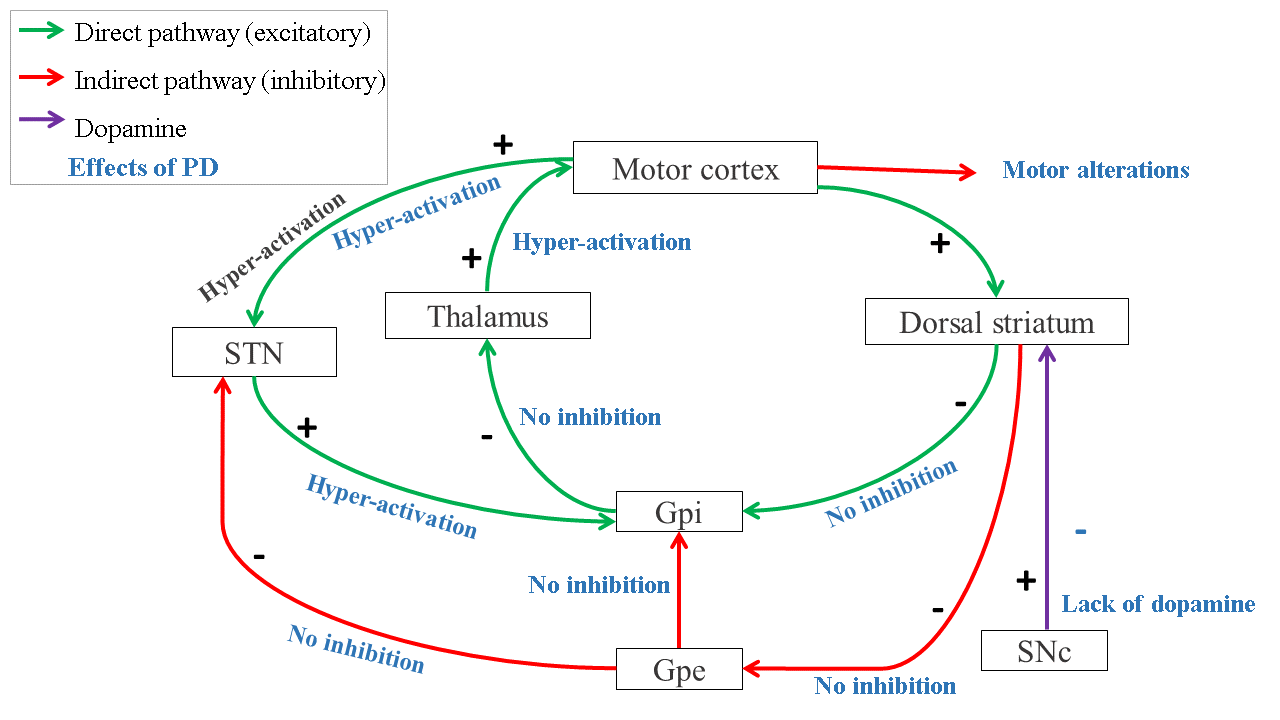
\includegraphics[width=0.9\textwidth]{basalGangliacircuit.png} 
       \caption{Neural network between main basal ganglia structures with connecting pathways inhibitory, in red, and excitatory in green. Alterations on pathways in PD patients are indicated in blue.}
     \label{fig:basalGanglia}
\end{figure} 

Parkinson's Disease is characterized by progressive degeneration of neurons in substantia nigra pars compacta (SNc), decreasing the secretion of dopamine (DA), an essential brain monoamine which regulates the excitability of striatal neurons. 
Effects of loss of DA lead to alterations in neuronal activity resulting in difficulties for movement control and are present both in indirect and direct pathways, as indicated in blue in  figure \ref{fig:basalGanglia}. Consequently GPi is inhibited and increases inhibition signals in the thalamus, finally hyper-activating the motor cortex and consequently inhibiting the control of voluntary movements \cite{Maiti2017}.% that hyper-ac which and results in inhibition of voluntary movement control, in motor cortex.  
\\

\textbf{Treatments for Parkinson's Disease}

Different therapies are currently available for the treatment of motor symptoms in PD. At the present, both medication and surgery are the most frequently used therapies to treat PD symptoms ((or decrease progression)), but new promising treatments are emerging and  being studied such as stem cell transplantation or gene therapy \cite{Maiti2017}.

During early stages of PD treatment, medication typically is the best option to control motor symptoms. Most common used drug is Levodopa (L-dopa) which is a dopaminergic drug that decreases the SNc degeneration by improving its dopamine levels. Nevertheless, since increment of dopamine occurs in other brain regions beyond the basal ganglia, it may generate adverse effects, specially in long-term treatments, such as motor fluctuations or dyskinesias. Also other types of drugs are used in PD treatment to treat motor (dopaminergic and non-dopaminergic drugs) and non-motor symptons.

For patients with motor symptoms refractory to the best medical therapy different therapeutical approaches are tried: usually deep brain stimulation or lesion surgery. 
 Lesion surgeries for PD are known as pallidotomy and thalamotomy referring to the respective surgically destroyed part, globus pallidus and thalamus. Motor symptoms decrease with these procedures since inhibitory neural activity of these estructures was increased. Nevertheless, since lesion surgery is irreversible and lesions in adjacent areas may occur, electrical neuro stimulation surgery (Deep Brain Stimulation) is a good alternative and currently most commonly used for PD.
 
%Motor fluctuations, change between states of regarding the control of motor symptoms. "off-time", "on-time"

\subsection{Deep Brain Stimulation}

Deep Brain Stimulation (DBS) is a surgical treatment for refractory movement disorders, such as PD, dystonia or tremors. A target area of the brain is stimulated through surgically-implanted electrodes to reverse motor symptoms by inducing neuronal activity alterations.

\begin{figure}[!htb]
     \centering    
         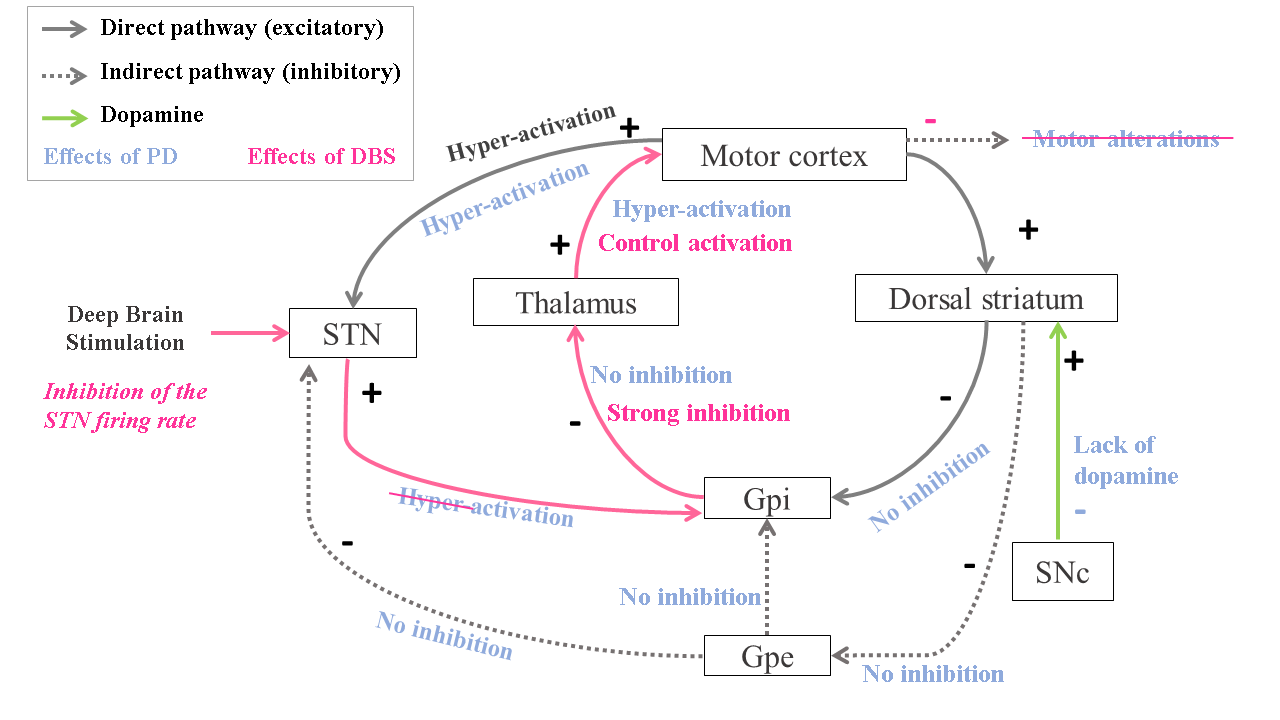
\includegraphics[width=0.9\textwidth]{basalGangliacircuitDBS.png} 

       \caption{Basal ganglia circuitry with alterations induced by STN-DBS in both indirect and direct pathways. Alterations to both inhibitory and excitatory pathways in PD patients are indicated in blue.}
     \label{fig:basalGangliaDBS}
\end{figure}

Our study is focused on STN-DBS and therefore our stimulation target is STN, typically used for PD treatment along with GPi. Up to 20\% of PD patients are considered suitable candidates for Deep Brain Stimulation (DBS),\textit{ since DEVELOP ABOUT CANDIDATE CONDITIONS FOR DBS?.} \cite{WagleShukla2014}.
% paf 45 vaz 

%\cite{Hamani2017} \cite{Tysnes2017}
%Condiciones para ser candidato para PD: pagina 45 vaz

Mechanism underlying STN-DBS can be explained following with the basal ganglia circuitry, figure~\ref{fig:basalGanglia}, altough it is still fully unclear how mechanism underlying STN-DBS exactly work within the brain. As illustrated in the basal ganglia neural network in figure~\ref{fig:basalGangliaDBS}, artificial stimulation in the hyper-activated STN provokes an inhibition of its firing rate that activates the GPi, consequently inhibiting the thalamus and improving movement control from motor cortex \cite{Maiti2017, Gradinaru2009, Negida2018}.

Subthalamic Nucleus is divided into three functional regions: sensorimotor, limbic and associative, which are located in dorsolateral, anteroventral and medial territories respectively, and it is part of a bigger functional structure called the basal Ganglia as mentioned before. Previous studies suggest that precise positioning of the electrode and stimulation within the sensorimotor part of the STN is of mayor importance for optimal results and to avoid side effects \cite{Castrioto2014, Wodarg2012, Johnsen2010}. However, identification of sensorimotor STN region based on 1.5 Tesla MRI images is impossible and still unclear based on MER characteristics.

\textit{Outcomes?}

\subsubsection{DBS procedure}
Previously to surgery and stereotactic frame implantation, pre-operative magnetic resonance imaging (MRI) is acquired in order to subsequently plan the lead trajectory based on the patient's anatomy. After installation of stereotactic frame, pre-implantation contrast-enhanced computed tomography (CT) is performed on patient, which displays a reference scale through its ferromagnetic materials.

Estimation of STN target coordinates is based on both CT and MRI pre-operative images co-registered and its fiducial points, AC (anterior commisure) and PC (posterior commisure).  For both hemispheres (one at a time), different trajectories and strategies are discussed and visualized to achieve the best trajectory based on merged images in both three views (sagital, coronal, axial) and also as \textit{probe view}, which facilitates avoiding problematic trajectories. Best electrode's trajectory avoids white matter, critical cerebral tissue, veins or other conflict points.

Once target coordinates are selected, surgery is performed one hemisphere at a time. Stereotactic frame is configured according to the target coordinates and after burr hole trepanations, electrodes are connected and implanted into the brain according to the fixed coordinates in the frame. In our study using Medtronic 3389 electrodes, only central, lateral and anterior leads were implanted but up to 7 leads in each electrode are available to use.

Registration of micro electrode recordings (MER) is next performed in order to identificate STN and therefore the best position based on acquired signals from different depths. MER start when electrodes are positioned one centimeter above the planned target, and recordings are acquired at different depths to target simultaneously for all the channels, located with a parallel trajectory to the center lead. \textit{(Through Medtronic console )}
According to the acquired signal and based on visual inspection and experience of the neurologist, region of brain in which the electrode is located for each depth is identified in a table. After registration of all depths, kind of a reconstruction of the shape of the target is estimated based on MER annotations and possible definitive target coordinates are determined.
 
Intraoperative stimulation is then executed in order to refine the final localization of lead based on therapeutic and side effects assessment. Different estimated points of interest are stimulated through inserted macro-electrodes with gradual variations of both intensities and frequency. Once stimulation effects, such as eye or muscle contractions, are assessed and the best position is determined, definitive electrode is implanted.
 
Second part of surgery includes the implementation of the neurostimulatter with the battery in the patient and its connection to the electrodes as illustrated in figure 1.1 \cite{Medtronic2007}. Batteries may need to be replaced in 3 to 5 years depending on the patient and stimulation parameters. 

\begin{figure}[!htb]
     \centering    
         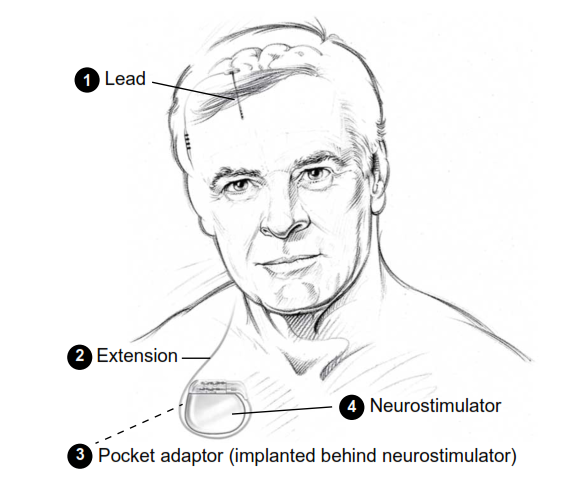
\includegraphics[width=0.6\textwidth]{medtronicDBScomp.png} 

       \caption{Medtronic DBS System Components. \small{From Medtronic.}}
     \label{fig:medtronicDBS}
\end{figure}

\textit{Develop about DBS programming??}

\subsection{Electrophisiology or action potentials}
\label{sec:electroph}
Explaining STN localisation and typical waveforms through different parts of the brain?
Also differences between patients and characteristics in PD (STN) or is it better in the discussion?

\subsection{Classification}

\section{Objectives}
\label{sec:objectives}
Development of clinical-support tools for identification of the target area in DBS is important for this field. As mentioned before, positioning of final electrodes in the precise location is related with the best therapeutic results and its definition depends on the neurologists expertise among other factors, so it is a time-consuming and subjective process. In this study we aim to contribute to the development of computational tools that can assist clinical decision in target identification in STN-DBS. Therefore, we split our objectives into four main tasks:

\begin{enumerate}
\item Development of an unbiased unsupervised tool for signal processing, analysis and feature extraction to distinguish STN from non-STN intraoperative MER, but easily adaptable for other types of signals and regions.

\item Development of an automatic approach for spike sorting and signal analysis of human brain MER to study physiological properties of neurons. We aim to construct this tool generalizable to other brain regions and unsupervised through the adjustment of existing algorithms to our approach.

\item Identification of features that distinguish sensorimotor subdivision of STN vs. limbic and associative using extracted features from both previously constructed tools.

\item Development of a hybrid unsupervised/supervised machine learning classification approach that uses extracted MER features for high-accuracy identification of STN. This approach can be optimized using individual patient lead trajectory localization reconstruction based on imagiology, fused with an STN functional subdivision atlas.
\end{enumerate}

\section{Contributions} % Introduction

\chapter{Methods}

In the present chapter, the dataset provided for the analysis is first explained. Then, procedures for labelling each MER are detailed followed by the pre-processing approaches for MER to clean the signals. Methodology for extraction of features, both directly from signal and from neuro-physiological information (spikes), are described in sections~\ref{sec:spkFeat} and~\ref{sec:tfnFeat}.  and constracted tools related is explained in the following sections.  

\section{Microelectrode Recordings}

	Our signals dataset was collected from 5 PD patients undergoing bilateral STN-DBS using three electrodes in each hemisphere -central, lateral and anterior channels. Recordings started 10 mm above the estimated target and ended approximately 3.5 mm after, thus signals were acquired at around 23 different depths in each channel, as shown in figure \ref{fig:datasret}. Acquisitions were sampled at 24 kHz per channel, filtered (band-pass filtering, 0.5-5 kHz) and amplified, previously to their storage. Duration of recorded signal varies between patients, since two of the patient's registers lasted for 30 seconds of duration at each depth while the rest of the recordings lasted for 10 seconds.
	
\begin{figure}[!htb]
     \centering    
         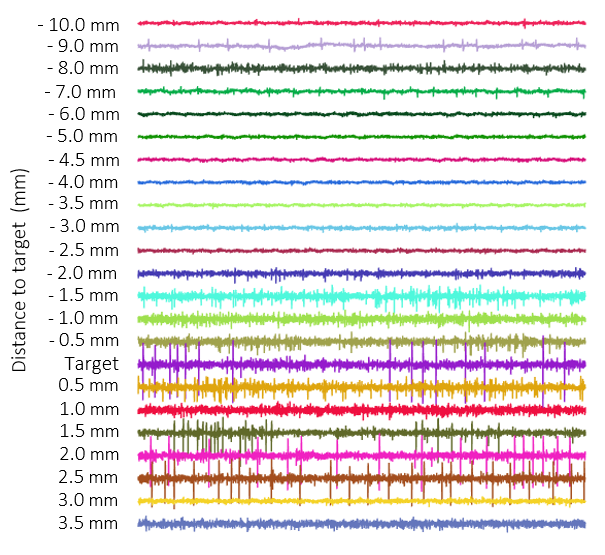
\includegraphics[width=0.7\textwidth]{depthsRN.png} 

       \caption{Segments of MERs (500 ms duration) at each depth along the trajectory with central electrode, starting recordings from 10 mm above target to 3.5 mm under.}
     \label{fig:datasret}
\end{figure} 

\textit{Table with patients data is important and where?. }
\subsection{Imagiology}

\textit{Is it necessary to describe provided\textbf{ images details and target coordinates in Z} here or is it better only in anatomically-based classification section???}


\section{Localisation of electrode position for MER labelling}

Labelling each MER of our dataset regarding its position is important in order to effectively identify features for distinguish STN from non-STN MER and to  to construct the automatic classifier. Therefore, different approaches are explored for labelling MER regarding its location within the target, both further explained in the following sections. First approach is based on unbiased visually inspection and classification of MER segments within STN by an expert. Second labelling is based on lead trajectory localization reconstruction using individual patient imagiology, fused with an STN functional subdivision atlas. Gold-standard classification could be obtained through this approach and it allows us to compare physiological neurons properties in motor/non-motor STN.

%\textit{Labelling each signal regarding its position in relation to the STN is essential. Thefore, all recordings are identified and labelled through two different approaches: visual inspection by an expert and based on patient's fused imagiology. Both procedures are further explained following.  Both approaches are further explained}



%Labels of STN subterritories, and gold standard labelling is based on 

%Neuroimaging
%Regarding the assesment of the 
%Patiet's magnetic resonance imaging (MRI) is studied in order to evaluating the patient's 
%defined labels and based on trajectory localization reconstruction
% acquired along the intraoperative trajectory are 

%Furthermore, in this study  patient's imagiology is also used to identify each localization of the microelectrode recordings along their trajectory. This data is important in order to correctly classify ----------
%Therefore, gold-standard classification of could be obtained through this approach and it allow us to based on patient's imagiology. 
%\subsection*{Localisation of electrode tip within the area of interest}
%Datos sobre la localizacion del electrodo en cada una de las señales son esenciales para la construccion de un classificador automatico. Por lo tanto 


\subsection{Expert-based classification}

Labels regarding each signal's position within the STN were identified  through visual inspection by an expert. In order to facilitate visualization and labelling of all signals and to preserve the classification unbiased to previous knowledge about MER depths, a customized script in Matlab was programmed. 

This script first shuffles all signals in the dataset and it plots in random order one signal at a time. The whole signal and two enlarged segments (1 second and 500 milliseconds duration, randomly chosen from the raw signal) are shown to classify, as shown in figure~\ref{fig:classifSgignals} for each signal in the dataset. Then, the expert is asked to identify the current signal as \textit{STN (1)}, \textit{not-STN (2)} or \textit{try again (3)}. If any signal is classified as \textit{try again} for the first time, it is shown again until the third attempt, when it is classified as \textit{unclear (3)}. 

Additionally for each signal classified as STN, the expert is asked to set its value of certainty of its localization from 1 (very unclear) to 5 (high certainty), which gives an idea of the confidence of each classification for further analysis.
 
\begin{figure}[!htb]
     \centering    
         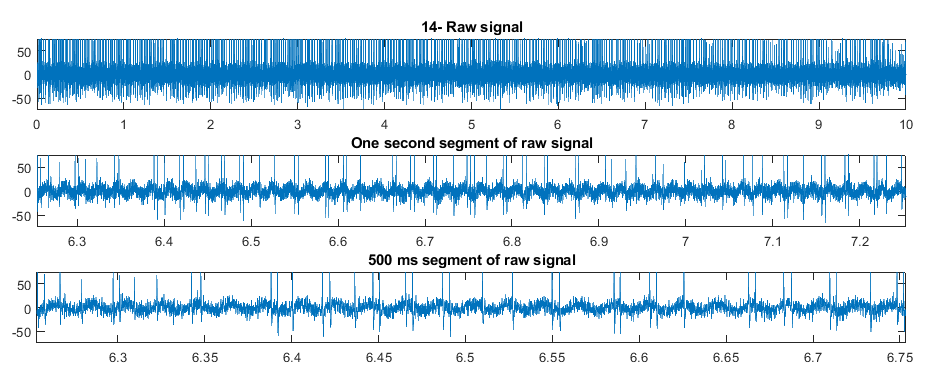
\includegraphics[width=0.7\textwidth]{selectionSignals.png} 

       \caption{Segments of MERs (500 ms duration) at each depth along the trajectory, starting recordings from 10 mm above target to 3.5 mm under.}
     \label{fig:classifSgignals}
\end{figure} 

\textit{Numbers of classification results (table) should be shown in results, right? } 
 
However, labelling subterritories of STN based on visual inspection is not a viable option since differences are not clearly discernible. Accordingly, this subdivision is manually defined by splitting the consecutive recordings identified as STN along each trajectory into three equal parts: dorsal, medial and ventral part of STN. Then, signals classified as borders of STN are discarded also with the medial ones, resulting in labels for both dorsal and ventral regions, probably motor and non-motor STN respectively. 


\subsection{Anatomically-based classification}

Reconstruction of trajectory localization for each lead presents a gold-standard approach, since it is based on both pre-operative and post-operative patient's imagiology fused to an atlas of STN functional subterritories. In order to localise the electrode tip and trajectory and also for patient's image processing, LeadDBS, a Matlab toolbox [\url{http://www.lead-dbs.org}; \cite{Horn2015}] were applied in this approach. Along with this software, Slicer3D [\url{https://www.slicer.org/}] is also used to import all images into Nifty, which were provided in DICOM.

Afterwards and through Lead DBS, MRI images are coregistered using SPM12 method [\url{http://www.fil.ion. ucl.ac.uk/spm/software/spm12/}], whereas post-operative contrast-enhanced computed tomography (CT) image was coregistered to preoperative MRI images with Advanced Normalization Tools [ANTs; \url{http://stnava.github.io/ANTs/}]. All volumes are later normalized to standard stereotactic space (MNI; ICBM152 2009b non-linear asymmetric) using Dartel implemented in SPM.

\begin{figure}[!htb]
     \centering    
     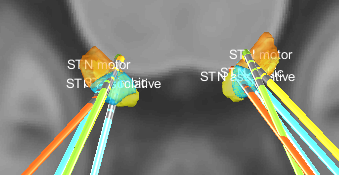
\includegraphics[width=0.7\textwidth]{stnReconstruct.png}
       \caption{Axial view of STN subdivisions with reconstructed electrodes based on each patient’s images through Lead DBS }
     \label{fig:spkSorting}
\end{figure}

In order to obtain electrode's location and trajectory, reconstruction is manually supervised assessed with pre-reconstruction through PaCER method and Acolla's STN subterritories atlas \cite{Accolla2014, Husch2018}. Once definitive coordinates of electrode are located, MER localizer tool in LeadDBS is used to determinate locations along the trajectory in all channels.

%Image specifications (acquisition) here? Lead DBS and Slicer methodology
%More accurate localization of recordings at each depth is estimated through reconstruction of the trajectory for each implanted lead with both fused pre-operative and post-operative patient's images and STN functional subdivisions \cite{Accolla2014} atlas.
%Reconstruction of trajectory will be performed through LeadDBS using STN subdivisions atlas reconstructed on patient’s 
%pre-operative MRI and pos-operative CT previously co-registered.
%Furthermore,  haciendo uso de (con recurso a) las fused images del pre and post operative images paciente se realizó otra classificacion, siendo asi considerada como gold standard. A través de estas señales y con la identificacion del posicionamento y el canal utilizado definitivo, se pueden obtener las diferentes posiciones de cada uno de los electrodos y canales along the route.
%Para esta classificacion se utilizo la toolbox de matlab Lead DBS software blabla, especializada ya en la reconstruccion de electrodos?
% Postoperative electrode reconstructions are performed using Lead-DBS toolbox [\url{http://www.lead-dbs.org}; %\cite{Horn2015}], implemented in Matlab. % [http://www.lead-dbs.org; Horn and K€uhn, 2015; RRID:SCR_002915] in Matlab.Along with this software, Slicer3D [\url{https://www.slicer.org/}] is also used to import all images into Nifty, which were provided in DICOM.
% of the  Una vez obtenida la localizacion definitiva del electrodo, la herramienta MER recoerdings? es utilizada para determinar la localizacion de los otros dos canales con trayectoria paralela utilizados (anterior y lateral) y asi obtenemos el posicionamiento para cada uno de nuestras profundidades y 
%Exporting DICOM images into Nifty performed com recurso a Slicer 3D. Postoperative electrode localizations were performed using Lead-DBS software % [http://www.lead-dbs.org; Horn and K€uhn, 2015; RRID:SCR_002915] in Matlab.
%First, MRI images were coregistered using SPM method () whereas post-operative CT was coregistered to preoperative MRI images with ANTs.
%Afterwards, volumes were normalized with SPM Shoot???.
%In order to obtain electrode's location and trajectory, reconstruction is manually supervised assessed with pre-reconstruction through PaCER method.

\section{Filtering MER and artefact detection}
\label{sec:filtering}
Some noisy signals are present in MER dataset with different types of artefacts. According to \citeA{Bakstein2017}, noise in MER may affect more than 25\% of the recording length and can arise due to a number of factors such as mechanical movement manifested by high power signal peaks, electromagnetic interference such as the 50 Hz interference from the power grid, low-frequency interferences ($<$50 Hz) and "irritated neurons" with high spiking activity. Consequently, pre-processing these signals is an important step in order to avoid errors in the extracted features and .

Filtering the signal is our first step in this pre-processing part, since it can smooth out high-frequency fluctuations and/or remove periodic trends of a specific frequency from data. Therefore we filter the data using an elliptic band-pass filter between 300 and 5000 Hz. Elliptic filter was chosen after visual inspection of different types of signals and its effects on spike detection, since it keeps waveforms of firing neurons unaltered \cite{QuianQuiroga2009}. Implemented filter of order 4 is set to 0.6 decibels (dB) of peak-to-peak ripple and 60 dB of attenuation and it is performed with zero-phase digital filtering in order to preserve time features. Nevertheless, all parameters can be easily modified in our tool and also code for testing other types of filters is implemented.

\begin{figure}[!htb]
     \centering    
              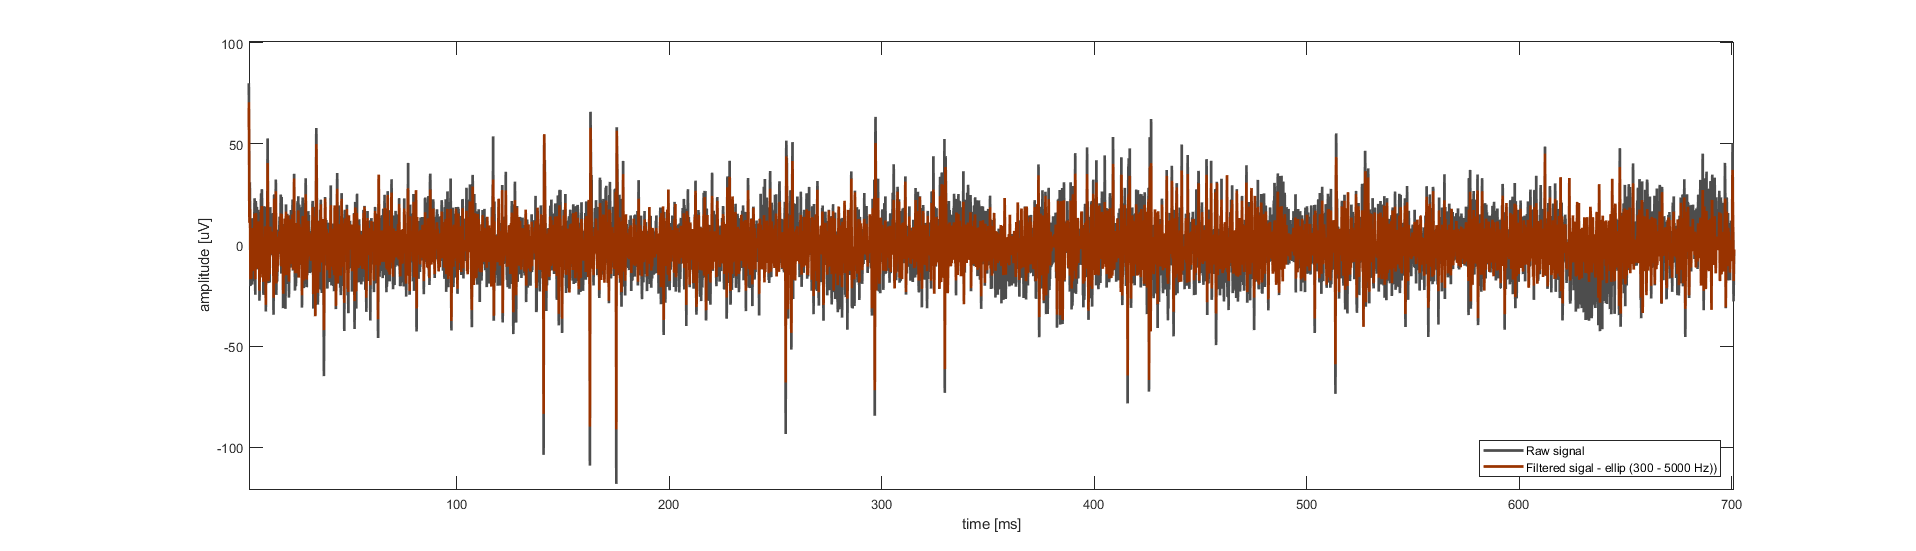
\includegraphics[width=0.7\textwidth]{filtered_700ms.png} 
       \caption{Filtered signal (700 ms) with elliptical filter overlapped to raw MER.}
     \label{fig:artifacts}
\end{figure}

In addition to the filtering, we reviewed previous approaches for MER artifact removal literature and visually inspected their performances on our dataset \cite{OShea2017, Bakstein2017, Grubhoffer2016}. Best observed approach for artifact detection was found with autocorrelation-based method from \citeA{Bakstein2017}. We  adapted their open-source algorithm in order to extract both the longest consecutive segment and a clean signal with the detected artefacts cropped? out, as illustrated in figure~\ref{fig:artifacts}

\begin{figure}[!htb]
     \centering    
       \caption{Reconstructed electrode trajectory with STN subdivision atlas}
     \label{fig:artifacts}
\end{figure}



\section{Extraction of features related with time, frequency and noise}
\label{sec:tfnFeat}

Differences between raw signals along the trajectory to target are discernible through visual inspection as shown before, therefore signal characteristics calculated through computational analysis might reflect these variations. Consequently features related with time, frequency and noise are extracted from filtered MER in order to find features for distinguishing STN from non-STN recordings.

Custom Matlab code was implemented to first load the table dataset with all MER data used, since following analysis and feature extraction is performed one signal at a time and extracted values for each signal are stored in a table along with recording data, all in an unsupervised way after setting input parameters. 

For each MER, the raw signal is first filtered as explained in section~\ref{sec:filtering} and then, if artefact detection and removal is performed, it is inspected and it results in a segment of cleaned signal from interferences. 

Segment of MER to analyse (or whole signal) is divided in smaller segments to extract its characteristics based on statistics of all segment's calculated features. This division in frames should provide a more robust approach for signals with noisy signals or high variability within the same signal vs. extraction of characteristics from the whole signal. Therefore, we split the signal into frames of 2048 samples overlapped 50\% (1024 samples) with Hanning windows, resulting in more than 230 segments for each 10 second signal (sampled at 24 kHz). 

Features related with time are then obtained directly from each frame: \textit{mean absolute value} (MAV), \textit{mean absolute value slope} (MAVS), zero crossings (ZC), \textit{RMS power} (Prms), \textit{waveform of curve length} (WL), \textit{variance} (var), \textit{Teager energy} (TE) and \textit{crest factor} (CrF). In relation to noise, two measures were obtained:an estimation of \textit{standard deviation of noise} (spN) and \textit{signal-to-noise ratio} (SNR). Features related with frequency domain are: \textit{spectral centroid} (spC), \textit{spectral roll off} (sRO), \textit{spectral flux}, \textit{mean frequency} (mFreq), \textit{median frequency} (medFreq) and \textit{12 Mel coefficients}. Features definition and formulas of extracted parameters are presented in appendix X.
% filtered MER divided in smaller segments through a custom Matlab code. Secondly, features based on neuronal activity from firing neurons, shown in MER as spike events as in figure 2, are calculated. Beforehand, spike events are detected from filtered signal and since they may be originated from more than one different neuron, spike sorting is performed identifying one cluster for each neuron, based on their spike waveforms and selected features. Preliminary probability tests with some extracted features show significant differences, as illustrated in figure 3 for STN identification and figure 4 regarding dorsal STN. 

\section{Features related with neuronal activity }
\label{sec:spkFeat}
Microelectrodes register neuronal activity, part of which consists of action potentials (AP), spikes generated from neurons in the nearest region of the electrode tip as already mentioned in section~\ref{sec:electroph}. Therefore, different depths of the brain show different neuronal activity and consequently, related characteristics are studied based on the detected spikes to extract relevant neurophysiological properties for target identification in STN-DBS.

Nevertheless, prior to the spike-related features quantification, action potentials of the different neurons are detected from the MER as spiking events by a process known as spike detection, further explained in section~\ref{sec:spkDetection}. Afterwards, different neurons are separated in different clusters, process detailed in section~\ref{sec:spkSorting} known as spike sorting. Extraction of their features is implemented lastly, once neurons are sorted and detected from each MER.

%\subsubsection{Spike features}
\textit{Algorithms for Spike Detection and Sorting. Should I explain them in detail? And here or in discussion/results when talking about modified parameters?}

\subsection{Spike detection}
\label{sec:spkDetection}
In this process, firing neurons are detected as spike events from the filtered signal. The used algorithm is Spike Detection with Continuous Wavelet Transform \cite{Nenadic2008}
 This algorithm uses the continuous wavelet transform (CWT) combined with information about the typical interval duration of AP to identify these spiking events. Biorthogonal family was used with this algorithm, though it can be used with other types of wavelets, but this family presents bi-phasic phase which is similar to APs, as illustrated in figure~\ref{fig:spkDetection}A,  and when translated and scaled, a bank of approximately matched filters for AP identification along the signal is formed.
 
\begin{figure}[!htb]
     \centering    
               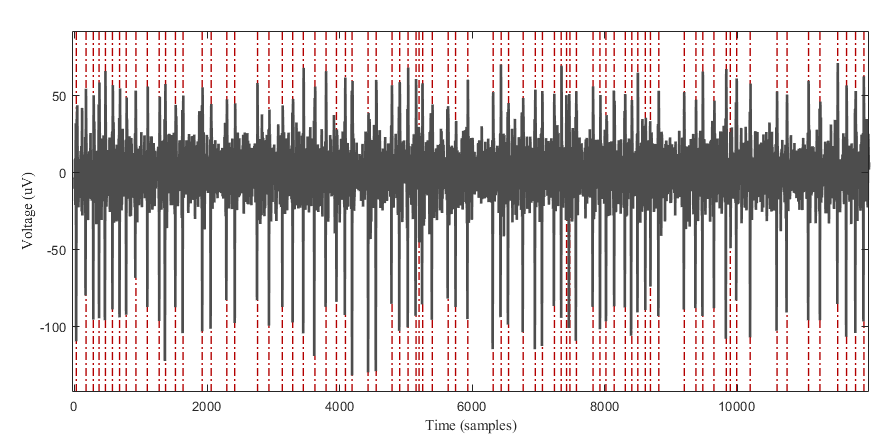
\includegraphics[width=0.9\textwidth]{spkDetection.png} 
       \caption{A)  Typical waveforms of action potentials (top) and biorthogonal wavelet family (bottom). B) Spike train of detected spike events (red) on the clean filtered signal (gray).}
     \label{fig:spkDetection}
\end{figure} 
 \textit{ Missing figure of wavelet vs. typical action potential shape! 
 Explain more deeply about wavelet or this algorithm?}
 
 Nenadic's algorithm was chosen instead of threshold detection, which is more widely used, since it presented better performance with an unsupervised approach on the number of detected spikes versus threshold detection (both fixed and adaptative) in noisy signals. This may be due to the fact that this method is less affected by the highly variability of amplitudes and background noise between all signals and more stable for unsupervised analysis. 
 
  \subsection{Spike sorting}
 \label{sec:spkSorting}
 Detected firing events within the same signal may be originated from more than one different neuron and consequently it is important to correctly identify their origin in order to avoid misclassifications and errors in the spike related features. Thus and as mentioned before, spike sorting consists in grouping the detected spikes into clusters based on the similarity of their waveforms.

Since we aim to develop an unsupervised tool for neurophysiological features extraction based on MER, we research the spike sorting literature in order to find a suitable algorithm to adapt to our analysis tool. Therefore our spike sorting is performed with Linear Discriminant Analysis and Gaussian Mixture Model (LDA-GMM) and outlier detection, through an available algorithm and implemented code in Matlab from \citeA{Keshtakaran2017}. 
This method using subspace learning applies LDA to extract most discriminative features from the spike waveforms and performs clustering with automatic detection of the number of the clusters based on GMM.
(Write more about LDA GMM).
Parameters adjustment (since used parameters were not defined by default...is explained better in results and mentioned here?)

\begin{figure}[!htb]
     \centering   
      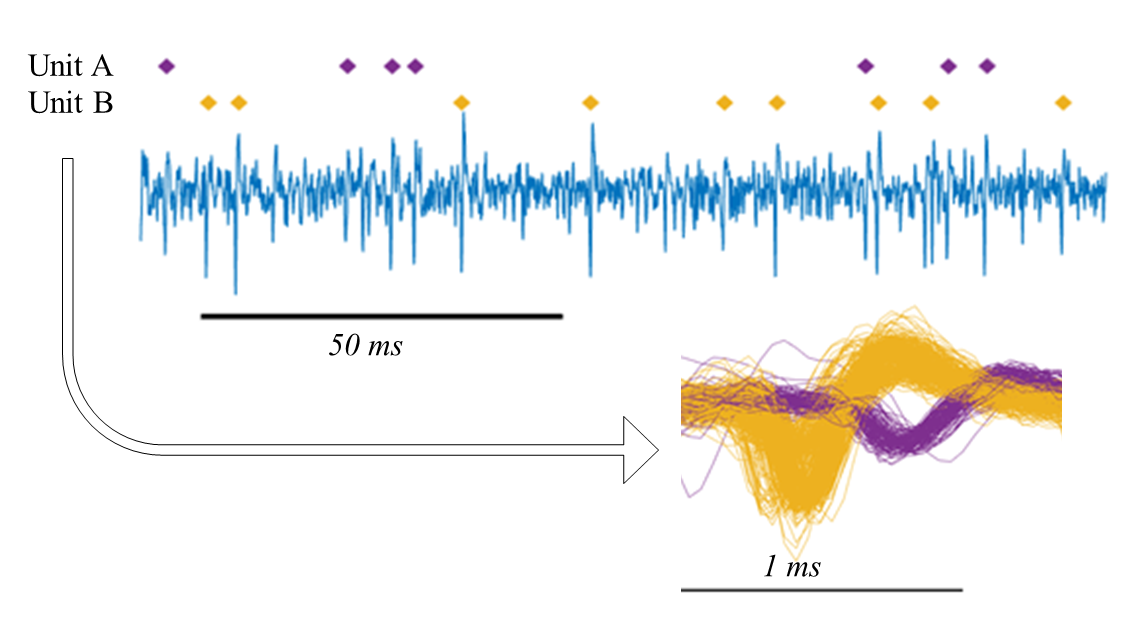
\includegraphics[width=0.75\textwidth]{spkSorting.png} 
       \caption{Detected spikes in filtered MER after spike detection and sorting (top) and their respective overlapped waveforms (bottom).}
     \label{fig:spkSorting}
\end{figure}  

In order to address the quality of each cluster in an objective and standardized way, different related measures are extracted through existing algorithms. Therefore and regarding the isolation quality for each cluster, isolation score is quantified as explained in \cite{Joshua2007}. This score measures the overlap between the noise and the spike clusters. Also with the same algorithm, an estimation of the proportion of false positive and false negative classification errors is obtained.

\subsection{Spike related features extraction}

Based on each neuron's spike train, related features are extracted again through custom Matlab code. Different groups can be distinguish with some of these characteristics according to the measurement unit related with. Specifically, three types of spike features are determined quantifying spike train oscillations, periodicity of spike trains and bursting-related neurons. 

In spite of these groups, \textit{Firing rate} is extracted as a measure of the number of spikes per unit.  \textit{Fano factor} quantifies the variability of the increments of a spike train, and it was calculated according to the literature \cite{Llc2005}. Median values of \textit{Spike maximum amplitude} and \textit{Spike peak-to-peak amplitude} are also stored as measurements of spikes events amplitude. 
 
 A group of features is based on periodicity of the spike trains, specifically related with the \textit{Inter-Spike Interval} (ISI).
%and consequently with the(?) Firing Rate (FR). 
 These features are \textit{Modified burst index} (MBI), \textit{Pause index} (PI), \textit{Pause ratio} (PR), \textit{Bursting index} (BI), \textit{Assimetry index} (AI), \textit{median ISI} (medISI) and \textit{coefficient of variation of ISI} (cvISI).
 
 Spike train oscillations characteristics are also studied through two different approaches. Since neuronal oscillations are typically separated into bands of frequency, these related features are also calculated for each range. Therefore, these bands of neuronal oscillatory activity are: delta (1–4Hz), theta (4–8Hz), alpha (8–12Hz), beta (12–30 Hz), and gamma (30–80Hz). \textit{Modulation indexes} and their significance are calculated through available algorithm and code \citeA{Matzner2015} . On the other hand, features quantifying the oscillation frequency and strength in the given band through the \textit{Oscillation score} and \textit{Oscillation frequency} through the method from \citeA{Muresan2008}.

\begin{figure}[!htb]
     \centering   

       \caption{Spike train and detected bursts through Rank Surprise algorithm}
     \label{fig:bursts}
\end{figure}  

Lastly, characteristics related with bursting neurons are calculated after bursts are previously detected through the Rank Surprise Algorithm, which is based on ISI for detecting bursts \cite{Gourevitch2007}. Extracted features from bursting neurons are: \textit{Burst rate} (BR), \textit{Burst duration} (BD), median \textit{Inter-burst interval} (interBI) and \textit{Intra burst frequency} (intraBI).


%De Vaz ECP: sincronizaçao dos circuitos provocada pela perda de dopamina relacionava-se com o aparecimento de um padrõ oscilarotio na banda beta (11-30 hz) qu era revertido com a alta frequencia na ecp e pela activaçao dopaminergica    ver pag 26 livro 


\section{Classification with Machine Laerning }
Automatic identification of the signals recorded in the Subthalamic Nucleus and specifically its sensorimotor part will be implemented trough machine learning techniques and using the previously extracted features also combined with the information of the electrode's localization for each depth along the trajectory to the area of interest.

%In order to identify these signals recorded from the STN and since multiple approaches are explored in the localisation and feature extraction, also different options and methods will be inspected to find the best classification performance to identify both the STN and furthermore, its motor subdivision. 
Nevertheless, this classification methods require both training and methodological testing and therefore big amount of data is necessary. It is in this matter mostly where your collaboration is essential for a good classification performance with high values of accuracy, sensitivity and sensibility.

Normalization of features?accros series using z-score
 % Introduction


\chapter{Results}
In the present chapter, results are explained by parts ...=IIKKf
maybe recording duration in table 2 is better here 

\begin{table}[htb!]
\centering
\caption{Characteristics of subjects, recording duration and number of MER depths.}
\label{tab:subjects}
\resizebox{\textwidth}{!}{%
\begin{tabular}{@{}cccccccc@{}}
\hline
 &  & \multirow{3}{*}{\begin{tabular}[c]{@{}c@{}}Age\\ at surgery\\ (years)\end{tabular}} & \multirow{3}{*}{\begin{tabular}[c]{@{}c@{}}Disease \\ duration \\ at surgery \\ (years)\end{tabular}} & \multirow{3}{*}{\begin{tabular}[c]{@{}c@{}}Years on\\  PD \\ medication\\ ?\end{tabular}} & \multicolumn{3}{c}{Intraoperative MER characteristics} \\ \cmidrule(l){6-8} 
\multirow{2}{*}{Patient} & \multirow{2}{*}{Sex} &  &  &  & \multirow{2}{*}{\begin{tabular}[c]{@{}c@{}}Duration\\ (seconds)\end{tabular}} & \multicolumn{2}{c}{Depths along trajectory to target} \\ \cmidrule(l){7-8} 
 &  &  &  &  &  & Right Hemisphere & Left Hemisphere \\ \midrule
 \hline
1 &  &  &  &  & 30 & 21 & 21 \\
2 &  &  &  &  & 10 & 25 & 24 \\
3 &  &  &  &  & 10 & 27 & 25 \\
4 &  &  &  &  & 30 & 22 & 23 \\
5 &  &  &  &  & 10 & 24 & 23 \\ \bottomrule
\end{tabular}%
}
\end{table}

\section{MER labelling}

Identification of MER localizations was performed based on visual inspection of the randomized dataset by an expert. 
Altough first option for MER labelling was to use the intraoperative annotations based on visual inspection during recording phase of DBS surgery, as in previous studies, this classification may be biased by the knowdledge of geometric locations.

STN was identified in 285 recordings in our dataset of 685 MER signals. As illustrated in table~\ref{tab:labelResult}, certainty of MER classification as STN varies between patients: 38 recordings were labelled with the maximum certainty levels in patient 4, whereas in patient 3 any MER was identified as STN.

DISC: This may be due to the electrode is actually not recording along the STN or to a missclassification in the visual inspection labelling.
Anatomically-based approach will help in refining our results with a gold-standard methodology and compare both classifications. 

\begin{table}[]
\begin{tabular}{lcccccccc}
\hline
\multirow{3}{*}{} & \multirow{2}{*}{\begin{tabular}[c]{@{}c@{}}Number \\ of MER\end{tabular}} & not-STN classified & \multicolumn{6}{c}{STN classified} \\ \cline{3-9} 
 &  &  &  & \multicolumn{5}{c}{Certainty} \\ \cline{5-9} 
 &  & Total & Total & \textless{}25\% & 25-50\% & 50-75\% & 75-95\% & \textgreater{}95\% \\ \hline
All patients & 702 & 417 & 285 & 70 & 60 & 36 & 66 & 53 \\ \hline
Patient 1 (AC) & 126 & 58 & 68 & 10 & 14 & 16 & 19 & 9 \\
Patient 2 (JAMN) & 144 & 119 & 25 & 9 & 4 & 5 & 5 & 2 \\
Patient 3 (LMST) & 156 & 113 & 43 & 14 & 25 & 3 & 1 & 0 \\
Patient 4 (RN) & 135 & 39 & 96 & 14 & 9 & 6 & 29 & 38 \\
Patient 5 (TM) & 141 & 88 & 53 & 23 & 8 & 6 & 12 & 4 \\ \hline
\end{tabular}
\end{table}

We compute the following results considering STN-MER when their certainty level of classification are bigger than 
\subsection{Expert based classification}

\section{Features related with time and frequency}


\subsection{Developed tool for feature extraction}

We developed a Matlab code for feature extraction with previous loading and preprocessing of MER. 

Since our approach computes features from each signal based on small segments of the signal, we expected artifacts not to influence very significantly in our results. Therefore, our first analysis of extracted features for distinguishing STN and non-STN recordings using this tool was performed calculating the median, mean and standard deviation of all frame values from  10 second segment filtered signal. Following results present 


compare statistics with both features in order to compare them. 




comparison performance with or without artefacts
-> small effect on final results due to ; etraccion de artefactos si seria mas relevante 


\subsection{Time domain features}

\subsection{Frequency domain features}

\section{Developed tool for neural MER analysis}

\subsection{Supervised spike sorting}
wave clus- sin embargo surgia el problema tras la inspeccion visual de que tanto en spike detection como en spike sorting a veces es necesaria supervision! en el propio articulo nos recomiendan laa supervision de los resultados calculados automaticamente y ajuste de la temperatura.

esto se nos sale de nuestros objetivos ya que queremos desarrollar una herram y ademas contamos con una cantidad muy grande de datos, supervisar todos los culsters seria demasiado demorado.

Sin embargo utilizamos Wave clus para comparar nuestro algoritmo adaptado y de alguna forma medir la accuracy de los cluster identificados, mostrado en seccion ,,

\subsection{Unsupervised developed spike sorting}
\textbf{Spike detection}
hablar de que este algoritmo nos permitio realizar una deteccion de spikes en señales en las cuales la identificaion era complicada 
\textbf{Spike sorting}

\subsection{Spike features extraction}
\textbf{ISI dependent features}
\textbf{Bursting related features}
\textbf{Oscillation features}

\subsection{Comparison of supervised vs. unsupervised spike sorting}

\section{Classification for STN identification}

For identification of STN we based only in tf featu since it is a fast approach which could be implemented on real time ...
\subsection{SVMclassifier}
\subsection{knn}
.....
\section{Features for STN subdivision identification}

\section{Refinement of MER labelling trough images}

expert based  This classification approach provides apermite tener nuestro dataset clasificado en relacion al area de interest y gracia a la aleatoriedad, el expert no esta biased por sus propias respuestas. Sin embargo, es un proceso demorado y podria estar sujeto a bastante subjetividad.

\subsection{Comparison expert vs. anatomically based classification}
Procurar un doente con erros na classification e mostrar la importancia de clasificar basandonos en la realidad

diagrama de 4 barras: stn(real) notSTN(real) stn anatomico que o marcelo disse que nao era subbtalamico(FP?) and FN

\subsection{Spike characteristics based on anaomically based...}

 % Introduction


\chapter{Discussion}


\chapter{Conclusion}

\appendices

\chapter{Features related with time and frequency}

\begin{enumerate}

\item Mean Absolute Value (MAV)

mav=sum(abs(f(1:end,:)))/win; %abs()

\item Mean Absolute Value Slope (MAVS)

mavs=[mav(:,2:end)- mav(:,1:end-1) zeros(size(mav,1),1)];

\item Zero Crossing (ZC)

zc=sum((f(2:end,:).*f(1:end-1,:))<=0)/(win-1);

\item Power RMS (Prms) 

$prms=sqrt(sum(f.^2))/win;$

\item Waveform of Curve Length (WL) 

wl=sum(abs(f(2:end,:)-f(1:end-1,:)));

\item Variance (var)

varf=var(f,[],1);

\item Amplitude Distribution Kurtosis (AKUR)?????

kurt=kurtosis(f); %%PROBLEMAS AQUI COM NaN

\item \textbf{Amplitude distribution Skewness (ASKW)????}

skw=skewness(f);  %%PROBLEMAS AQUI COM NaN

\item \textbf{Crest factor (CRF)}

relation between peak amplitude and rms of the signal.
crf=(max(f(:,1:end))-min(f(:,1:end)))/2.*prms(1,1:end);

\item \textbf{Teager energy (TE)}
(Rajpurohit, 2014)
for i=1:size(f,2)
     Teager energy (Rajpurohit, 2014)
    $teaE(1,i)=(sum(f(2:end-1,i).^2-f(1:end-2,i).*f(3:end,i)))/(length(f)-2);$
    % Peaks (Rajpurohit, 2014)
    %peaks(1,i)=numel(findpeaks(f(:,i),par.fsOut));

% Noise (Rajpurohit, 2014)
%three times the std of the amplitudes in the data window
\item \textbf{Standard deviation of noise (?NAME?)}%9.
estimação do std do ruído (é o scale parameter da pdf)
calcular hilbert transf.
$fi=hilbert(f);
f_env=abs(f+fi*sqrt(-1));$
sdt do ruído estimado com mediana: mediana=sP*sqrt(2*ln2)
$spn=median(f_env)/sqrt(2*log(2));$


\end{enumerate}

\section{Frequency related features}
 % Appendix with features definition



\newpage

%\printbibliography
\bibliographystyle{apacite}
\bibliography{memoria_ref}
%\bibliographystyle{apacite}
%/Users/-sara/Documents/BibTex/draft_references.bib}

\end{document}